% !TEX root = ../main.tex

\section{Sensitivity analysis}

A Sobol sensitivity analysis of the Debiagi pyrolysis kinetics in a batch reactor model was performed using 9,000 samples which represent a range of biomass compositions (see Figure \ref{fig:sa-param-values}). A reaction time of 10 seconds, a reactor temperature of 773.15 K (500$^{\circ}$C), and a reactor pressure of 101,325 Pa were applied to the model. Batch reactor yields generated from the samples are shown in Figures \ref{fig:batch-sa1} and \ref{fig:batch-sa2}. The most pronounced gas trends are observed for the lignin-o, tannin, and triglyceride concentrations while liquids appear to be most affected by triglycerides. The greatest affects on solid yields seem to be from tannin and triglyceride concentrations.

\begin{figure}[H]
    \centering
    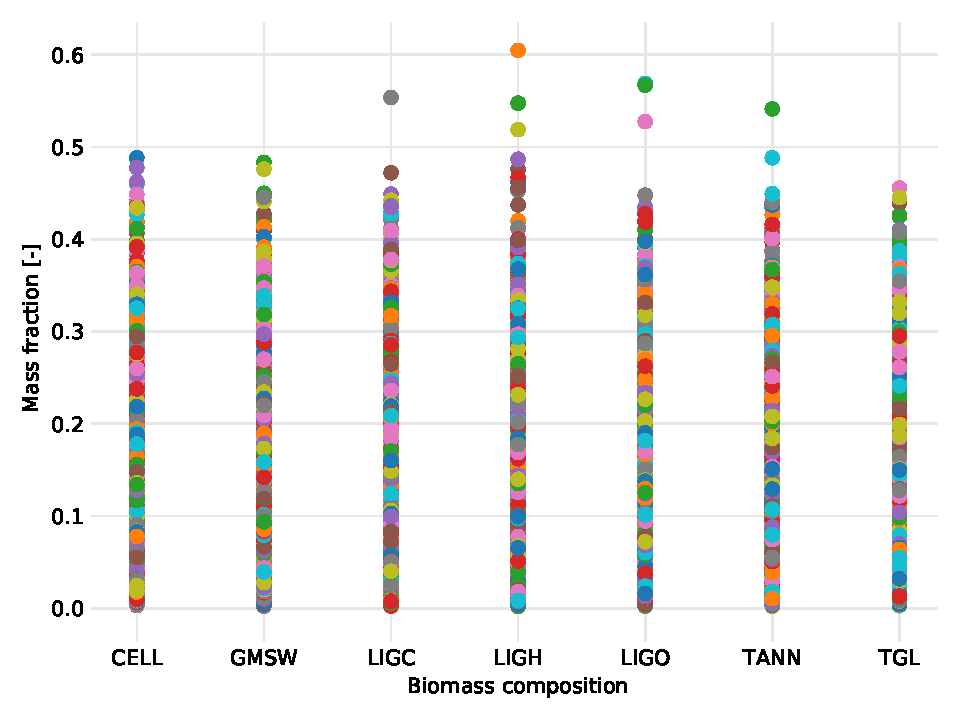
\includegraphics[width=0.8\textwidth]{figures/sa-param-values.pdf}
    \caption{Parameter values (biomass composition) used for input to batch reactor model. The values represent 9,000 samples used for the sensitivity analysis.}
    \label{fig:sa-param-values}
\end{figure}

The Sobol sensitivity analysis based on the batch reactor results is presented in Figure \ref{fig:batch-sa3}. Sobol indices from results with and without thermodynamic effects (heat of reaction) are shown in the figure. The results from the first-order indices (S1) are discussed below. Similar results are observed for the total-order indices (ST). Similar trends were observed between the non-thermodynamic and thermodynamic results; however, the difference between the first-order and total-order indices was more pronounced for the thermodynamic results.

\begin{itemize}
    \item gas yields are most affected by lignin-o, tannins, and triglycerides
    \item liquid yields are most affected by triglycerides and tannins
    \item solid yields are most affected by tannins and triglycerides
\end{itemize}

\begin{figure}[H]
    \centering
    \makebox[\textwidth][c]{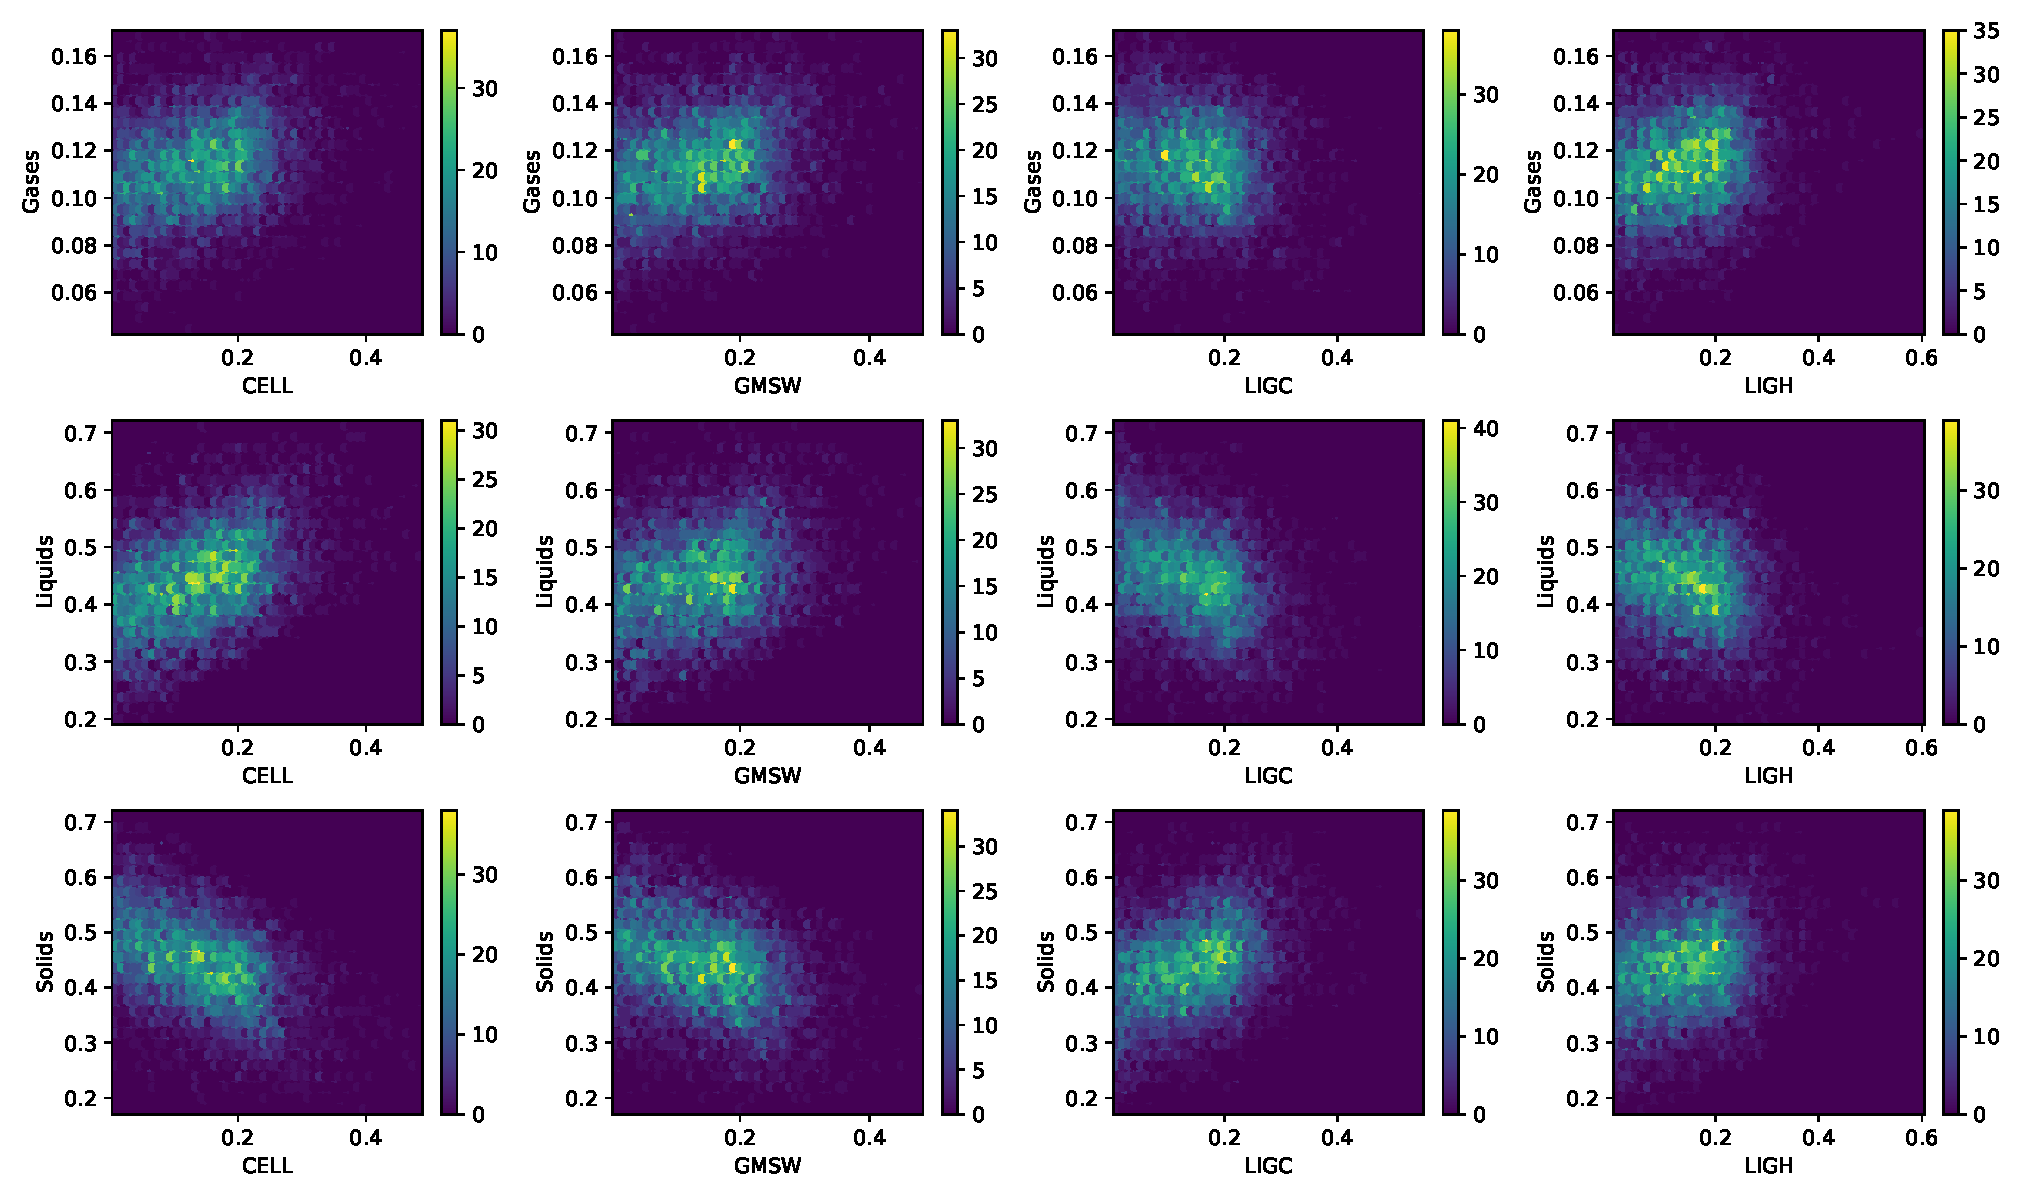
\includegraphics[width=1.3\textwidth]{figures/sa-hexbin1-n1000.pdf}}
    \caption{Batch reactor results for cellulose, hemicellulose (GMSW), carbon-rich lignin (LIGC), and hydrogen-rich lignin (LIGH) using 9,000 samples. Reaction time is 10 seconds at 773.15 K without thermodynamics. Colorbar represents bin count.}
    \label{fig:batch-sa1}
\end{figure}

\begin{figure}[H]
    \centering
    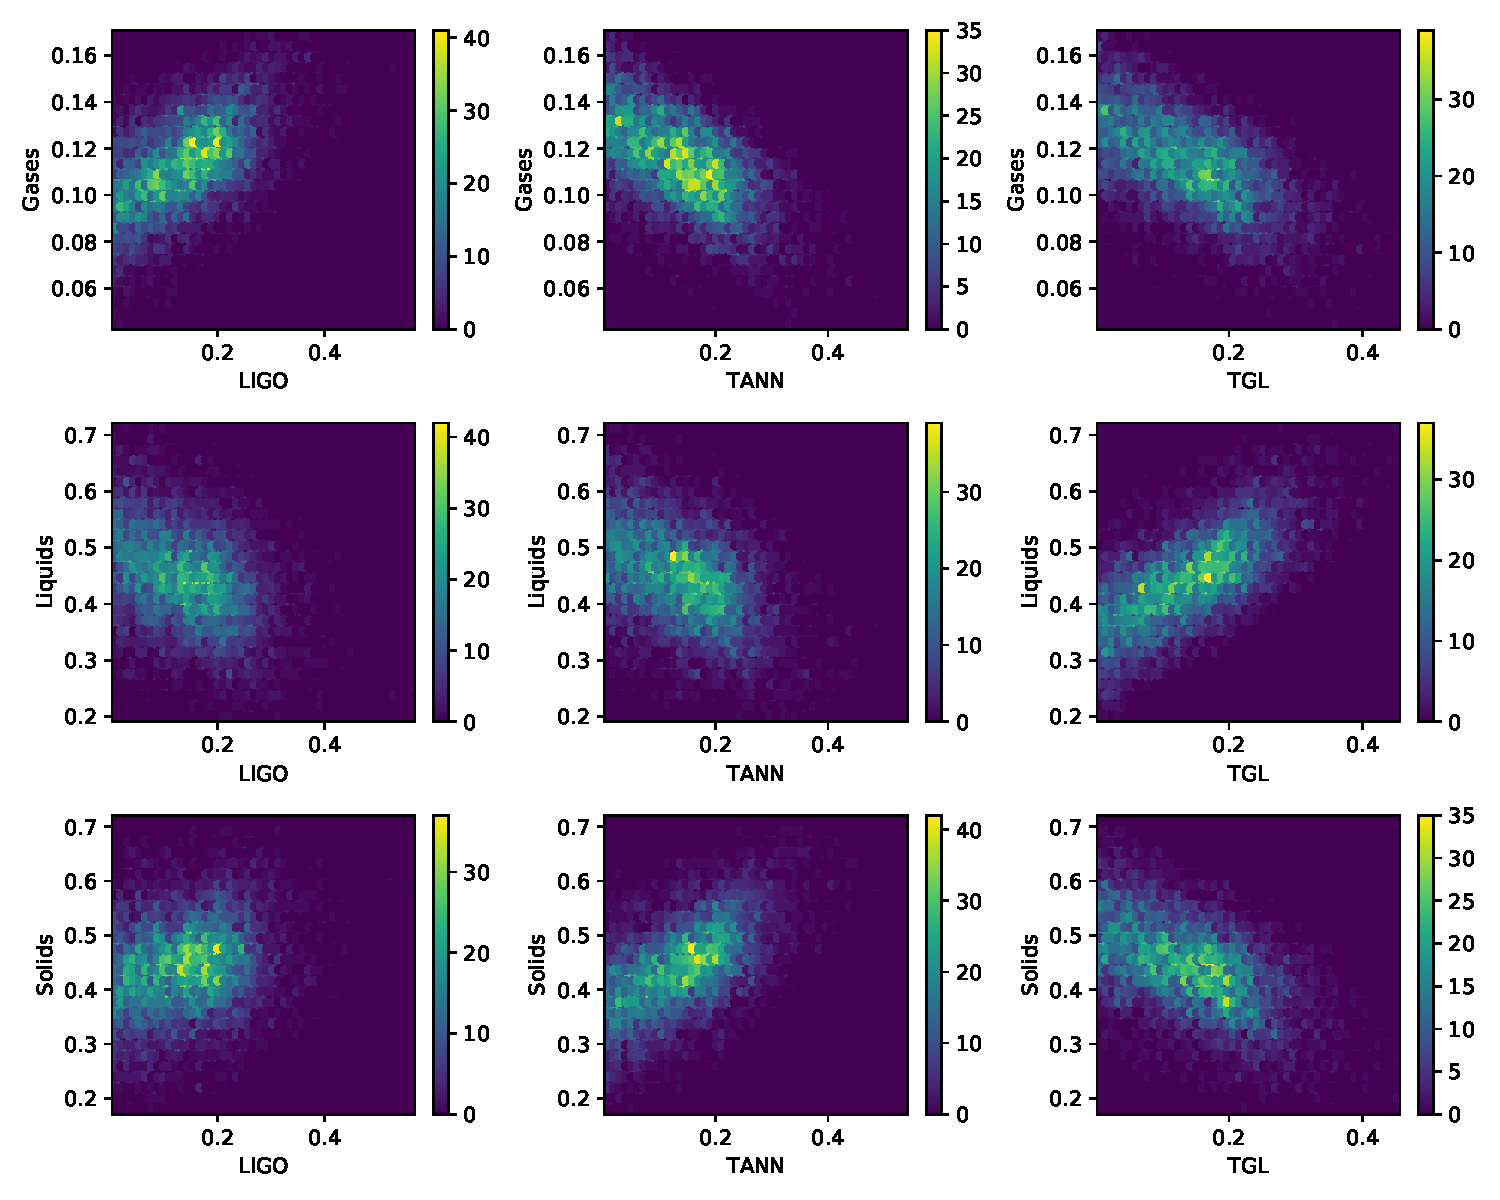
\includegraphics[width=\textwidth]{figures/sa-hexbin2-n1000.pdf}
    \caption{Batch reactor results for oxygen-rich lignin (LIGO), tannins (TANN), and triglycerides (TGL) using 9,000 samples. Reaction time is 10 seconds at 773.15 K without thermodynamics. Colorbar represents bin count.}
    \label{fig:batch-sa2}
\end{figure}

\begin{figure}[H]
    \begin{subfigure}{\textwidth}
        \centering
        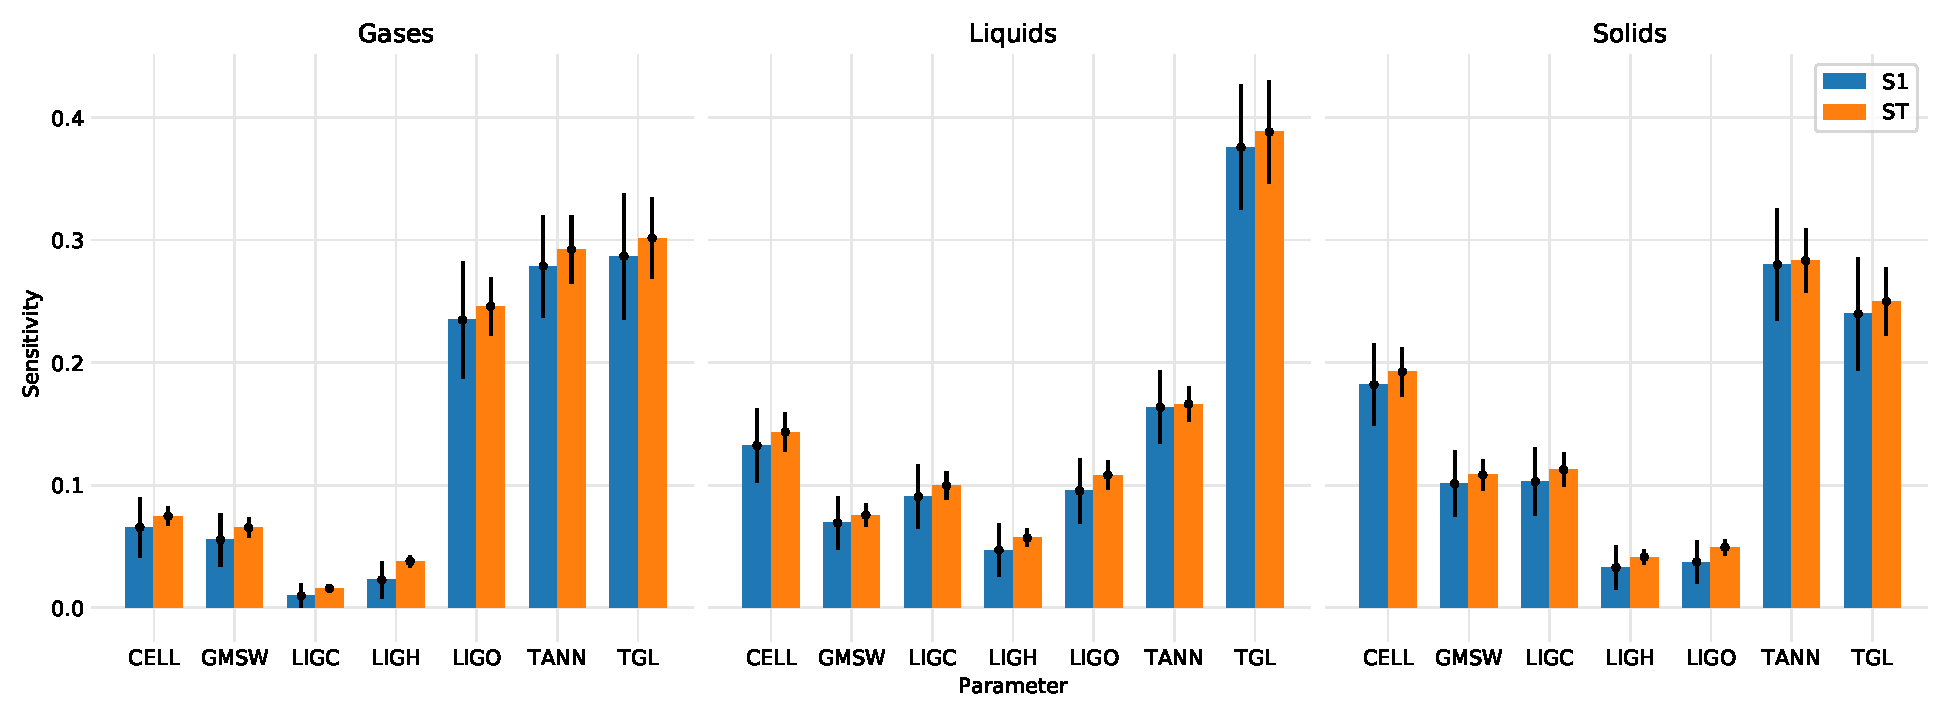
\includegraphics[width=\textwidth]{figures/sa-bar-n1000.pdf}
        \caption{Without thermodynamics.}
    \end{subfigure}
    \begin{subfigure}{\textwidth}
        \centering
        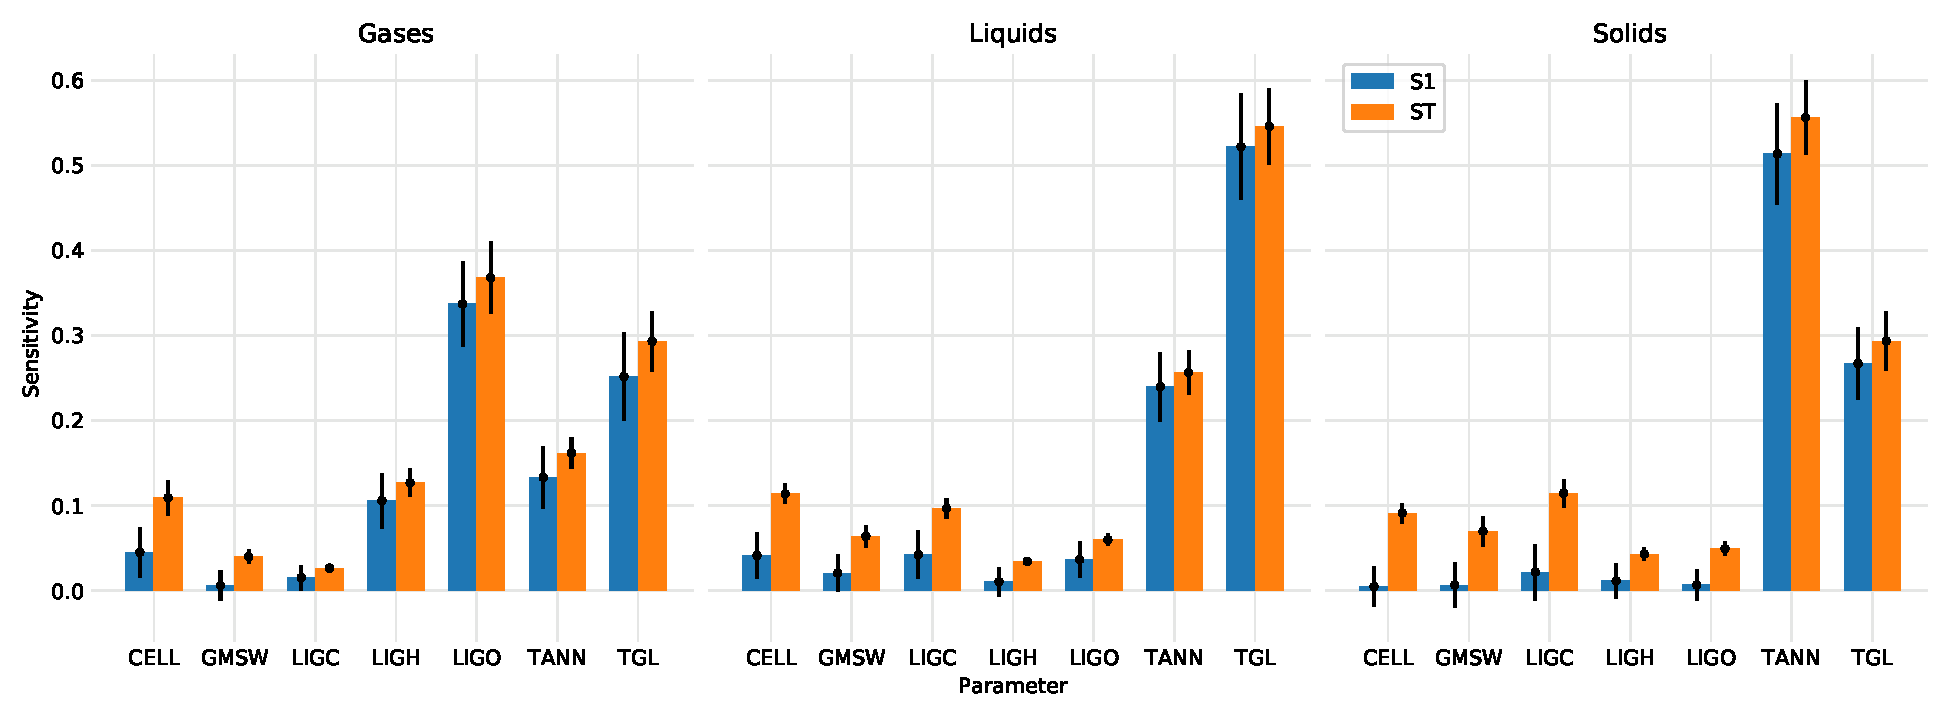
\includegraphics[width=\textwidth]{figures/sa-bar-n1000-energy.pdf}
        \caption{With thermodynamics.}
    \end{subfigure}
    \caption{First-order (S1) and total-order (ST) Sobol indices for biomass composition with pyrolysis reactants grouped as gases, liquids, and solids using 9,000 samples.}
    \label{fig:batch-sa3}
\end{figure}
